\documentclass[12pt,a4paper,oneside,twocolumn]{article}

\usepackage{fancyhdr} %Paket laden

%Umlaute ermöglichen
\usepackage[utf8]{inputenc}

%Einstellungen der Seitenränder
\usepackage[left=2cm,right=2cm,top=0cm,bottom=5cm,includeheadfoot]{geometry}

% Verwendung von Farbbefehlen
\usepackage{color}

% Um Bilder wie Logos einzubinden
\usepackage{graphicx}
% Um Text um Bilder herum zu legen
\usepackage{wrapfig}

%neue Rechtschreibung
\usepackage[ngerman]{babel}

\usepackage{enumitem}

% Um 1/2 2/3 etc darstellen zu können Verwendung: \sfrac{1}{2}
\usepackage{xfrac}

% Tabellentuning
\usepackage{multirow}
\usepackage{tabularx}
\newcolumntype{R}{>{\raggedleft\arraybackslash}X}%
\renewcommand{\arraystretch}{1.8} % Tabellenzeilenabstand

% Eigener Kopf-Fußzeilen Stil
\pagestyle{fancy} %eigener Seitenstil
\fancyhf{} %alle Kopf- und Fußzeilenfelder bereinigen
\fancyhead[L]{\Large Projektvorstellung: SABI - Seawater Aquaristik Business Intelligence} %Kopfzeile links
\fancyhead[C]{} %zentrierte Kopfzeile
% \fancyhead[R]{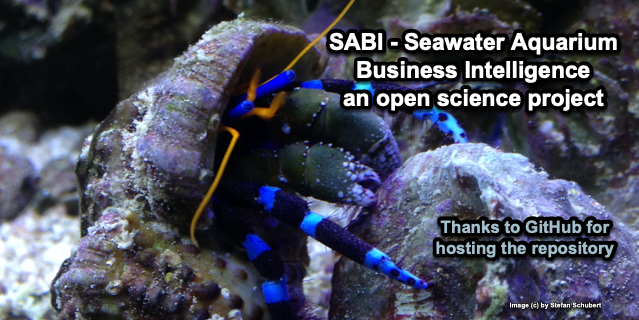
\includegraphics[angle=0,totalheight=42pt]{RepositoryPreview.png}\vspace*{-0.2cm}} %Kopfzeile rechts
\renewcommand{\headrulewidth}{0.8pt} %obere Trennlinie
\fancyfoot[C]{\thepage} %Seitennummer
\renewcommand{\footrulewidth}{0.8pt} %untere Trennlinie

% Grüne Header und Footerlinien
\definecolor{sabiblue}{rgb}{0,0.25,1}
\renewcommand{\headrule}{\vbox to 6pt{\hbox to\headwidth{\textcolor{sabiblue}{\hrulefill}}\vss}}
\renewcommand{\footrule}{\vbox to 6pt{\hbox to\headwidth{\textcolor{sabiblue}{\hrulefill}}\vss}}
\setlength{\headheight}{128pt}

%Bestimmte Trennungen vorgeben
% Gleichzeitig wird bei Wörten mit "-" die Regel aufgehoben, dass nur dort
% getrennt werden darf. D.h. hyphenation würde dann nicht zur Anwendung kommen.
\usepackage[T1]{fontenc}
\hyphenchar\font=\string"7F
\hyphenation{
Java
Software-entwicklung
Programmier-sprachen
Datenbank-systeme
Server
}

\begin{document}



% Autor-Kurzdaten
\begin{flushleft}

{\it Zum Autor} \\
\begin{minipage}[t]{\linewidth}
\begin{wrapfigure}{L}{0.4\textwidth}
{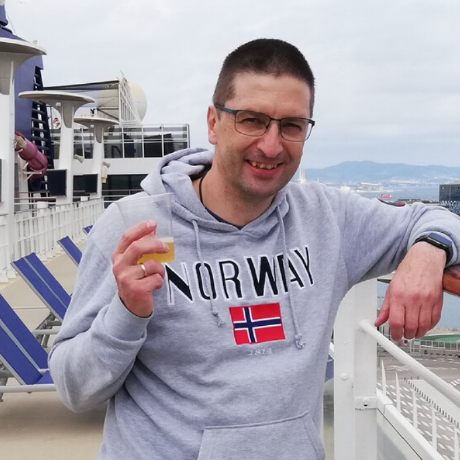
\includegraphics[scale=0.2]{Autor.png}}
\end{wrapfigure}
Stefan Schubert ist Diplom Informatiker und arbeitet IT-Berater. Den Einstieg in die Aquaristik fand er mit 16 Jahren im Süßwasserbereich. Über den Tauchsport entdeckte er seine Vorliebe zum Salzwasser und seit 2012 ist er begeisterter Nano-Reefer eines 80L Cubes.
\end{minipage}
\\
\vspace{0.5cm}
{\it Was ist SABI und welchen praktischen Nutzen haben Meerwasser-Aquaristiker davon?} \\
\vspace{0.5cm}


{\it Was bedeutet semi-wissenschaftlich?} \\
% \vspace{-1cm}


{\it Wie ist es zu dem Projekt gekommen? Was war die ursprüngliche Motivation } \\
% \vspace{-1cm}

{\it Wie kann ich am Projekt teilnehmen? } \\
% \vspace{-1cm}


{\it Was hat es mit dem ipv6 auf sich und weshalb lädt die Anwendung manchmal langsam? } \\
% \vspace{-1cm}

...privat Projekt / low budget / Bessere Infrastruktur, wenn Sponsoren...

% ========================== Sonstiges ======================
\textcolor{sabiblue}{\Large{Projektlinks}}
\vspace*{0.8cm}

\textcolor{sabiblue}{\normalsize{Zu Sabi}}\\
\vspace*{0.5cm}

{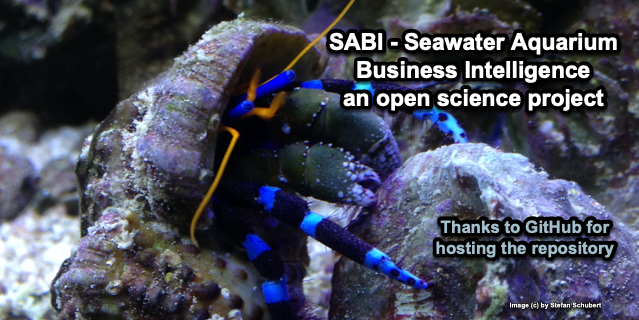
\includegraphics[scale=0.4]{RepositoryPreview.png}}\\
\vspace*{0.5cm}
WebAnwendung (im IPV6-Netz) | https://sabi-project.net\\
Für Entwickler zur Mitarbeit: | https://github.com/StefanSchubert/sabi\\

\vspace*{0.5cm}
\textcolor{sabiblue}{\normalsize{Infos zu IPV6}}\\
\vspace*{0.5cm}

Zur Anschlussprüfung | https://www.test-ipv6.com\\
Zur Verbreitung | https://www.google.de/ipv6/statistics.html\\
Für Bastler mit IT-Background | https://accso.de/magazin/ipv6-im-heimbereich/

\end{flushleft}
\end{document}